% !Mode:: "TeX:UTF-8"
\documentclass[runningheads,a4paper]{llncs}

%\usepackage{aaai17}
\usepackage{times}
\usepackage{helvet}
\usepackage{courier}
\frenchspacing
\setlength{\pdfpagewidth}{8.5in}
\setlength{\pdfpageheight}{11in}

\usepackage{showframe}%show the margin
%\usepackage{ulem}%used for uwave
\usepackage{comment}
\usepackage{subfigure}
\usepackage{enumitem}
\usepackage[ruled,vlined,linesnumbered]{algorithm2e}
\usepackage{algorithmic}

\usepackage{bm}%used for bm
\usepackage{graphics} % used for scalebox
\usepackage{graphicx}
\usepackage{amsmath} %used for maths symbols and the checkmark
\usepackage{amssymb}%used for empty set symbol
\usepackage{threeparttable} % used for footnotes in table
\usepackage{booktabs} %used for tnote
\usepackage{url} %used for url

\usepackage{makecell}

%Chinese
\usepackage{CJKutf8}
\inputencoding{utf8}

%================================================
%highlight
\usepackage{color,soul}%used for hl
\newcommand{\hlgreen}[1]{
	\sethlcolor{green}
	\hl{#1}
	\sethlcolor{yellow}
}%used for highlight, but set the color as green
%================================================
%================================================

%================================
%中文
\inputencoding{utf8}
\newcommand{\chinese}[1]{
	\begin{CJK*}{UTF8}{gbsn}
	#1	
	\end{CJK*}
}
%================================

\usepackage{multirow}% for table

\newtheorem{rmk}{Definition}% definition

%used for quotes
\usepackage{epigraph}
\setlength\epigraphwidth{\columnwidth}
\setlength\epigraphrule{0pt}

\usepackage{array}
\newcolumntype{L}[1]{>{\raggedright\let\newline\\\arraybackslash\hspace{0pt}}m{#1}}
\newcolumntype{C}[1]{>{\centering\let\newline\\\arraybackslash\hspace{0pt}}m{#1}}
\newcolumntype{R}[1]{>{\raggedleft\let\newline\\\arraybackslash\hspace{0pt}}m{#1}}

\usepackage{hyperref}
\setcounter{secnumdepth}{2}  
 \begin{document}
% The file aaai.sty is the style file for AAAI Press 
% proceedings, working notes, and technical reports.
%
%\title{Category-Level Transfer Learning from Knowledge Base to Microblog Stream for Accurate Event Detection}
\title{Leveraging Knowledge Base for Accurate Event Detection on Microblog Stream}
\titlerunning{Transfer Learning for Accurate Event Detection}
%构造(building)一个**词表(找一个词对它更合适的描述),for transfer learning in accurate event detection
%\title{Constructing Knowledge Base's Category Topics for Transfer Learning in Accurate Microblog Event Detection}
%\begin{comment}% for double blind
\author{Weijing Huang\inst{1} \and Wei Chen\inst{1} \thanks{Corresponding author.} \and Tengjiao Wang\inst{1} \and Yazhou Wang\inst{1} }
\institute{Key Laboratory of High Confidence Software Technologies (Ministry of Education), EECS, Peking University, Beijing, China \\ 
\path{huangwaleking@gmail.com,{pekingchenwei,tjwang}@pku.edu.cn}\\ 
\path{pkuwangyz@gmail.com}
}
%\end{comment}

\maketitle

\begin{abstract}
Many web applications need the accurate event detection technique on microblog stream. 
But the accuracy of existing methods are still challenged by microblog's short length and high noise. 
We develop a novel category-level transfer learning method \textsc{TransDetector} to deal with the task.  
\textsc{TransDetector} bases on two facts, that microblog is short but can be enriched by knowledge base semantically with transfer learning; and events can be detected more accurately on microblogs with richer semantics.
%文本短,建模很困难;直接做迁移学习困难,两者的组织结构不同,如何从精心构造的知识库迁移到微博是一个很大的挑战。
%所以我们提出了Category-Level Transfer Learning ...
The following contributions are made in \textsc{TransDetector}.
(1) We propose a structure-guided category-level topics extraction method, which exploits the knowledge base's hierarchical structure to extract categories' highly correlated topics. 
(2) We develop a probabilistic model CTrans-LDA for category-level transfer learning, which utilizes the word co-occurrences and transfers the knowledge base's category-level topics into microblogs. 
%Hence, word time series are expanded as category-pivot word time series.
(3) Events are detected accurately on category-level word time series, due to richer semantics and less noise. 
(4) Experiment verifies the quality of category-level topics extracted from knowledge base, and the further study on the benchmark \textit{Edinburgh twitter corpus} validates the effectiveness of our proposed transfer learning method for event detection.
\textsc{TransDetector} achieves high accuracy, promoting the precision by 9\% without  sacrificing the recall rate.
%另外,我们还标注了事件,使其语义可理解。以及LTDetector是efficient的。

\end{abstract}

\section{Introduction}
Many web applications need the accurate event detection technique on microblog stream, such as public opinion analysis\cite{thelwall2011sentiment}, public security\cite{Li:2012gw}, and disaster response\cite{Yin:2012ht}, etc.
Although event detection has been a research topic for a long while\cite{allan1998topic}, event detection in microblog stream is still challenging\cite{atefeh2015survey}.
According to \cite{huang2016probabilistic}, the characteristics of microblog, which is fast changing, high noise, and short length, raise the challenge.

Knowledge base can be a good supplementary for event detection on microblog stream.
Different from the not-well-organized microblog stream, knowledge base (e.g. Wikipedia) is constructed elaborately and contains rich information. 
For example, the microblog message ``Possible Ft. Hood Attack Thwarted (2011-07-28)'' is short, but still comprehensible because the words ``\textit{Ft. Hood}" is included in the wiki page ``\textit{Ft. Hood}", and belongs to the category ``\textit{Military}''.
By reading these two wiki pages, the model easily understands the example tweet is talking about something related to \textit{Military}.
In other words, knowledge base enriches the linkages between words, and provides more comprehensive context for microblogs.
Since the transfer learning\cite{pan2010survey} aims at utilizing the extra information restored in the source dataset to benefit the target dataset, it provides a feasible way to enhance the event detection in microblog stream.
%拆成两个小图,中间说明这是transfer learning过后的
\intextsep=3pt plus 3pt minus 1pt
\begin{figure}[h]
        \centering
        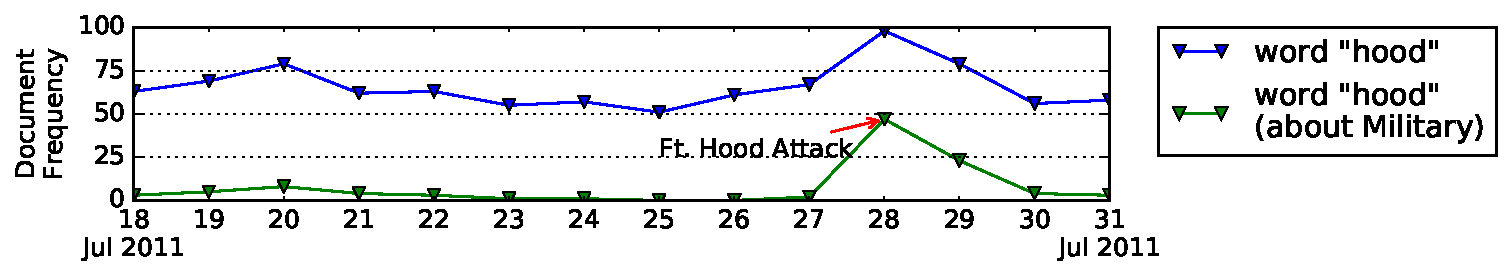
\includegraphics[width=1.0\columnwidth]{img/hood.pdf}
        %\caption{Hood\footnote{\url{https://en.wikipedia.org/wiki/Naser_Jason_Abdo#Arrest}}\footnote{\url{https://en.wikipedia.org/wiki/Fort_Hood#2011_attack_plot}}}
        \label{fig:hood}
\end{figure}



But it's non-trivial to conduct transfer learning from knowledge base to microblog stream directly.
The existing RDF model\cite{klyne2006rdf} lacks an efficient quick mechanism to transfer the knowledge, since it's mainly designed for managing knowledge as tuples on graph. And the query on large graph is also very expensive\cite{huang2011scalable}, which is not suitable for the scene of quickly and acuaretely detecting events.
What most meet the efficiency demand is Twevent\cite{Twevent2012}, but it's limited to filtering out meaningless microblogs by looking up Wikipedia. Some event,  which may contains the segments not restored in Wikipedia, may be dropped incorrectly.

In our paper, to balance the performance and the cost of transfer learning, new data structure \textit{KB states} is proposed. 
It bases on the following facts. 
The knowledge base's three fold structure includes the taxonomy graph (\textit{class} \(\rightarrow\) \textit{subclass}), the category-page bipartite graph (\textit{class} \(\rightarrow\) \textit{instance}), and the page-content map (\textit{instance} \(\rightarrow\) \textit{content}) relations in the knowledge base. 
In terms of concept level, the latter part is finer than the former. 
And the last page-content map goes into the detail at the word level. 
By considering these three parts together, we can extract a class or category's highly related words (evaluated by chi-square score in Section \ref{subsec:hs_initialization}), and restore them in the newly proposed data structure \textit{history states}.
In transfer learning, \textit{history states} play an important role at speeding up building the linkage between the word in microblog and the high level concept in knowledge base. 

More than that, we propose a new quick and lightweight probabilistic model KB-Prior-LDA for transfer learning. 
After deriving KB-Prior-LDA (detailed in Section \ref{subsec:rs_initialization}), it reveals that whether a word in microblog links to a high-level category in knowledge base depends on three factors, the word's score in the category's \textit{KB state}, the linkages of microblogs' other words, the linkages of the word types in the same time window. 
All these statistics are easy to gain, which leads the model efficient. 
What KB-Prior-LDA learned is summarized as \textit{recent states}, shown in Figure \ref{fig:modelDesc}.
Since the recent states have filtered out meaningless words, the detected events on recent states is much more accurate than other methods which don't do the transfer learning.
\textsc{KB-Prior-LDA}, \textit{history states}, and \textit{recent states} forms up our proposed event detection method \textsc{LTDetector}.
Our experiment on the real dataset \textit{Edinburgh twitter corpus (30 million tweets)} validates the effectiveness of our proposed method \textsc{LTDetector}.

\intextsep=5pt plus 3pt minus 1pt
\begin{figure}[h]
	\setlength{\abovecaptionskip}{0.cm}
	\setlength{\belowcaptionskip}{0.cm}
	\centering
    \label{fig:subfig} %% label for entire figure
        \subfigure[]{
                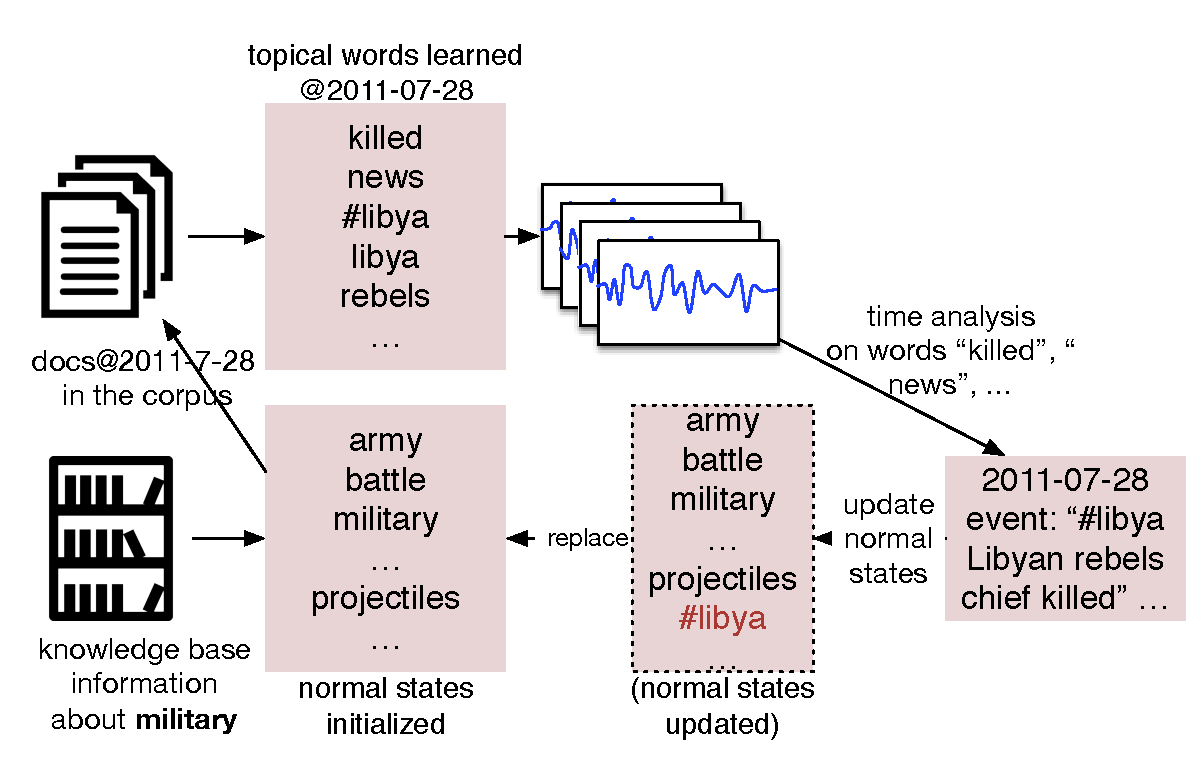
\includegraphics[width=.42\columnwidth]{img/NSDetectorExample.pdf}
                \label{fig:modelDesc}

        }
        \subfigure[]{
                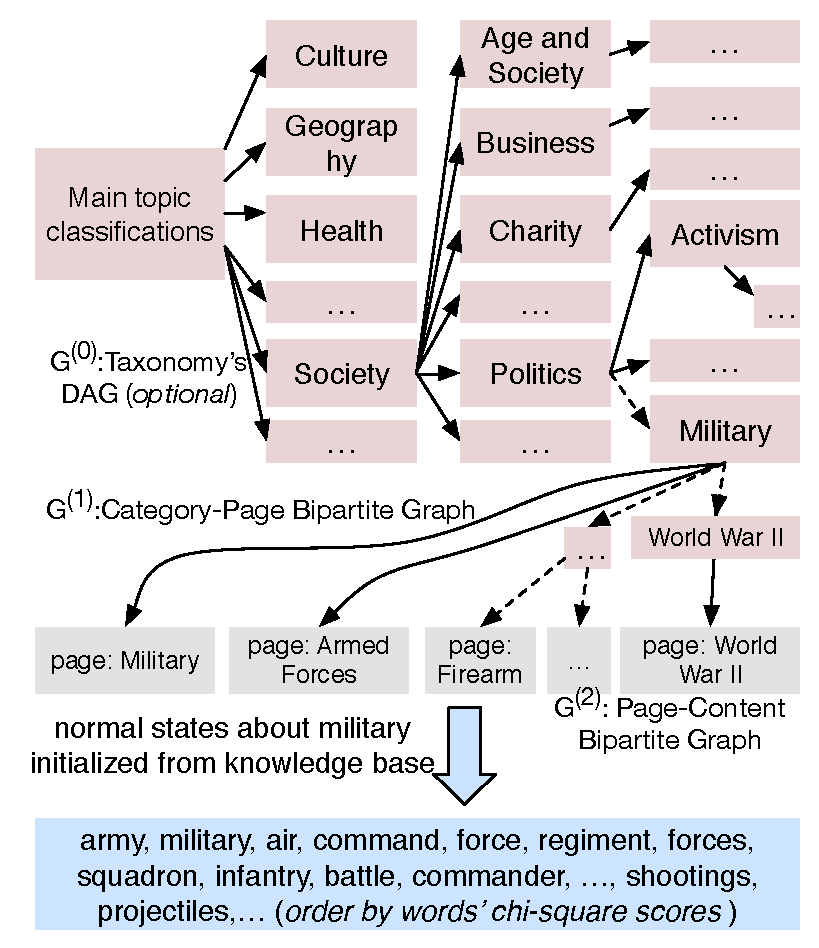
\includegraphics[width=.42\columnwidth]{img/initializationExample.pdf}
                \label{fig:NSinitializaton}
        }
        \caption{(a)\textsc{TransDetector}'s process flow, taking \textit{Military} related events in cyberspace as an example. \textsc{TransDetector} initializes the normal states about military from knowledge base, learns the topical words further within the time windows on the target corpus, detects events.;(b)Illustration on how to initialize history states from Wikipedia, taking \textit{Military} as an example.}
\end{figure}


%The contribution of this paper is mainly in three aspects.
%(1) We reveal that transfer learning from knowledge base to microblog stream can benefit event detection task.
%(2) We propose the probability model \textsc{NSDetector}. 
%The model can combine the history data and the recent data, further determine the arrival new document whether it represents a new event. 
%More than that, \textsc{NSDetector} has the capability to update the knowledge of what happened.
%(3) The experiment on the Edinburgh twitter corpus which contains 30 million tweets show that \textsc{NSDetector} promotes the accuracy rate by 9\% without sacrificing the recall rate.


\section{Related Works}
\label{sec:relatedWorks}
\textbf{Event Detection.} According to how much data are used, the approaches are divided into two groups: the detection \textit{without extra information}, and the detection by \textit{leveraging extra information}. 

Most existing methods are implemented \textit{without extra information}.
They utilize the bursty pattern in the text stream to detect events, and are carried out by  clustering articles\cite{Allan:2000wu,Petrovic:2010uj,Wurzer:2015wq}, analyzing word frequencies\cite{Mathioudakis:2010fc,Weng:2011wz}, or finding bursty topics\cite{Diao:2012wj,Yan:2015wm}. 
(1) By clustering articles, UMass\cite{Allan:2000wu}, LSH\cite{Petrovic:2010uj}, k-Term-FSD\cite{Wurzer:2015wq} and other similar methods model the occurred events as clusters of articles, and link the incoming article with an already existed event cluster or label it as the first story of a new event.
The decision is based on whether the dissimilarity between the incoming article and existed event clusters is over the user-specified threshold. 
Taking LSH as an example, as \cite{Petrovic:2010uj} discussed, the threshold controls the result: the big one leads to very few and broad clusters, while the small one results in very small and specific clusters.
Even after carefully set the appropriate threshold, the clusters generated by this kind method are still mixed of events and non-events due to large portion of non-event microblogs, which requires some post-processing methods as the supplement. 
(2) By analyzing word frequencies, TwitterMonitor\cite{Mathioudakis:2010fc} models the bursty words by queueing theory, and EDCoW\cite{Weng:2011wz} exploits wavelet transformation, which converts signal from time domain to time-scale domain, to detect the change point of word signal. 
However they treat the word as the most basic unit in analysis, without regarding how many concepts are represented by the word.
(3) By finding bursty topics via topic modelling, TimeUserLDA\cite{Diao:2012wj}, BurstyBTM\cite{Yan:2015wm} generates detected events.
TimeUserLDA distinguishes user's long term interests and short term bursty events, and BurstyBTM utilizes the burstiness of biterms as prior knowledge.
They both need to set the appropriate number of topics to run the topic modelling, and detect the ``large" events that associate with many articles but ignore the ``small" ones. 
To summarize, due to microblog's short length and high noise, it's not easy to set the directly applicable parameter for existing methods to achieve high precision and high recall simultaneously.

The second group methods detect events by \textit{leveraging extra information}. 
\cite{huang2016efficient} incorporates user's and the followees' profiles in microblog platform as the extra information for modeling user's long term interests, and further detects the bursty events which draws the attention of users with different interests. 
However many event detection scenes only provide the microblog stream without user profile information and the following network.
\cite{osborne2012bieber} compares two time series generated by event-related tweets and corresponding Wikipedia article's page views, and further filter out spurious events of microblogs.
Twevent \cite{Twevent2012} divides the tweet into segments according to the Microsoft Web N-Gram service and Wikpedia, then detect the bursty segments and cluster these segments into candidate events for necessary post processings.
But Twevent is still hampered by the performance of simply clustering the bursty segments shown by \cite{Yan:2015wm}.
If not limited to microblog stream, many systems also use the extra information for improving event detection.
\cite{steiner2013mj} utilizes the concurrent wikipedia edit spikes for event detection.
And \cite{liuleveraging2016} leverages the ACE corpus\cite{doddington2004automatic} and the structure of FrameNet\cite{baker1998berkeley} to improve the event detection within FrameNet, but has not shown how to apply the knowledge base for more general unstructured corpus.
In a nutshell, existing works are different from ours, as we transfer the category information of knowledge base into microblog's words and get the finer processing objects in event detection, rather than treating the knowledge base as a lookup table or a comparison base.
%Wikipop\cite{ciglan2010wikipop} uses the statistics of page views on Wikipedia articles to detect the personalized events.
%\cite{mcminn2013building} leverages LSH, wikipedia to build a large corpus for evaluating event detection on twitter.
%The unsupervised methods, including UMass\cite{Allan:2000wu} and BurstyBTM\cite{Yan:2015wm}, use \textit{the data within the recent time windows} to help to decide whether the incoming article is related to a new event. 


%The reason why this kind methods cannot achieve high precision and high recall simultaneously lies in that they lack the accumulation of history knowledge. 
%This kind methods ``understand" the document only by the recent data and the frequencies of the data, but the ``understanding" is not so confident that they still need the specific threshold to help to make decision. 

\textbf{Knowledge Base} Recently, many general knowledge bases and customized knowledge bases are constructed and utilized for different text mining tasks. 
For example, Probase\cite{wu2012probase} constructs a large general probabilistic \textit{IsA} taxomomy from webpages, and is used for semantic web search, and text classification\cite{wang2014concept}.
Such kind efforts are also made by DBPedia\cite{auer2007dbpedia}, Yago\cite{fabian2007yago}, and Freebase\cite{bollacker2008freebase}. 
These works manages knowledge as tuples on graph. 
However the query on large graph is very expensive\cite{huang2011scalable}, which is not very suitable for the scene of quickly and accurately detecting events.

The customized knowledge bases such as EVIN\cite{kuzey2014evin}, Event Registry\cite{leban2014eventRegistry}, and Story-base\cite{wu2015storybase}, are designed for managing events.
These knowledge bases are mainly built on news articles.
EVIN maps the existing event-related news articles into semantic classes. 
Event Registry collects the articles by the API of News Feed Service\cite{trampuvs2012newsfeed}, then detects events, and provides the structural information of the events, such as the related Wikipedia article, timestamp, and location etc. 
Storybase introduces Wikipedia current events\footnote{\url{https://en.wikipedia.org/wiki/Portal:Current_events}} as the resources for constructing event-and-storyline knowledge base on news articles, which are provided by GDELT project\cite{leetaru2013gdelt}.
As the news articles may lag behind the microblogs when the emergency of events, it's not enough to detect events from microblog stream by directly applying these customized knowledge bases. 



%近年来,知识图谱也被广泛应用在了文本挖掘领域,TKDE的文章利用wikipedia将



%Although \cite{Wurzer:2015wq} points out that UMass\cite{Allan:2000wu} and its variants\cite{Petrovic:2010uj}\cite{petrovic2012using}\cite{Wurzer:2015wq} are the state-of-art systems on the Event Detection task for the newswire data, these systems still suffers from the lack of accuracy to applied on more general cyberspace data, such as tweets, emails, and reddit posts. 

%\textbf{Knowledge Base}. \cite{faralli2015large} propose the Twixonomy Graph. 


%Twitter Trending Topic Classification
%We use PageRank-HITS\cite{Yan:2015wq} algorithm to update score of categories in wikipedia.

%3*4 figures, 0-11 is reorganized in the following order: 0, 1, 4, 5, 8, 9;
%2, 3, 6, 7, 10, 11;
\begin{comment}
\begin{figure*}[ht]
        \centering
        \label{fig:subfig} %% label for entire figure
        \subfigure[\((0.25,0.25,0.25)\)]{
                \label{fig:subfig:a} %% label for first subfigure a
                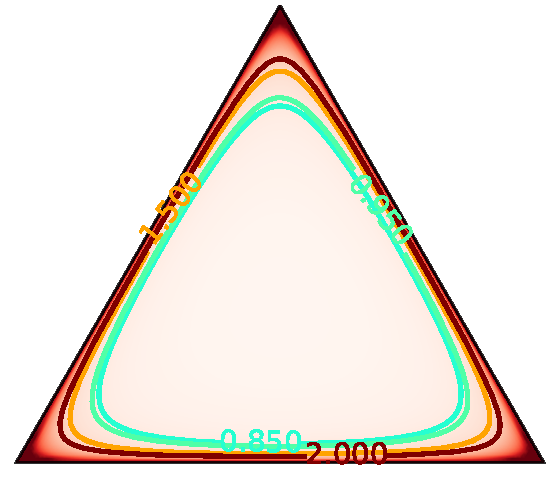
\includegraphics[height=2.14cm]{img/croppedDirichletGraph0.pdf}
        }
        \subfigure[\((0.5,0.5,0.5)\)]{
                \label{fig:subfig:b} %% label for second subfigure b
                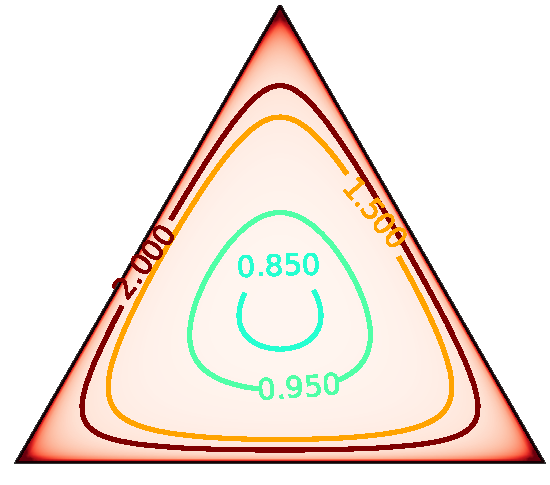
\includegraphics[height=2.14cm]{img/croppedDirichletGraph1.pdf}
        } 
        \subfigure[\((0.25,0.25,0.75)\)]{
                \label{fig:subfig:c} %% label for third subfigure c
                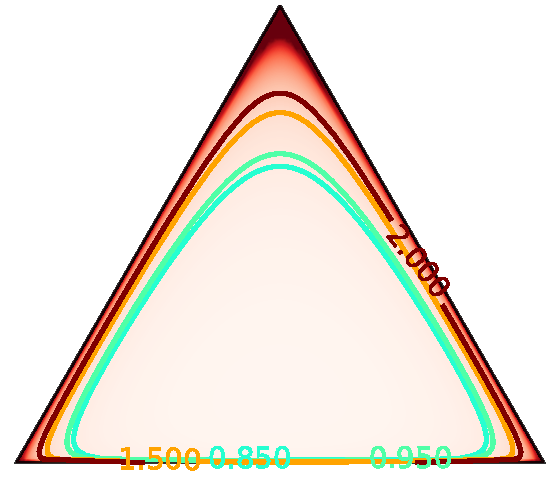
\includegraphics[height=2.14cm]{img/croppedDirichletGraph4.pdf}
        }
        \subfigure[\((0.5,0.5,1.5)\)]{
                \label{fig:subfig:a} %% label for first subfigure d
                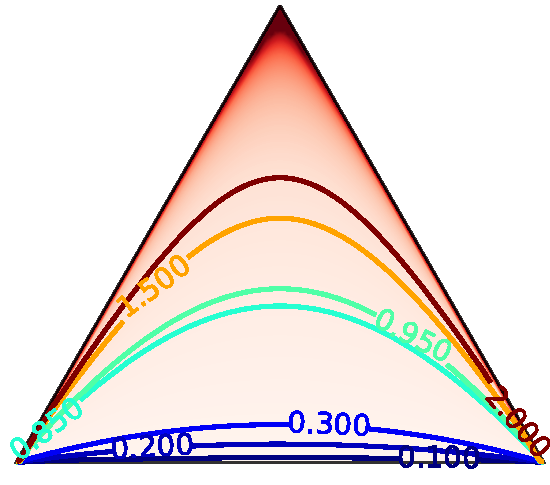
\includegraphics[height=2.14cm]{img/croppedDirichletGraph5.pdf}
        }
        \subfigure[\((0.25,0.75,0.75)\)]{
                \label{fig:subfig:d} %% label for third subfigure e
                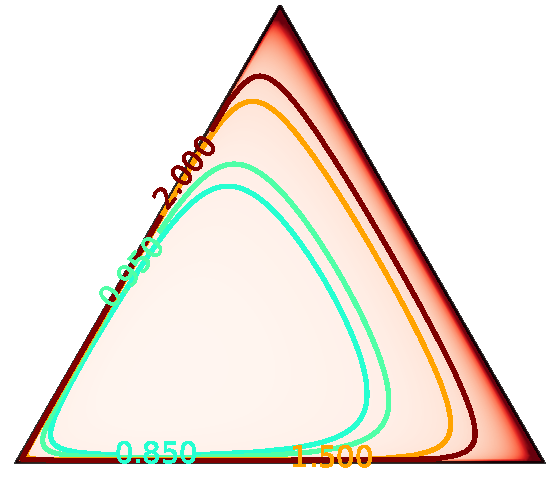
\includegraphics[height=2.14cm]{img/croppedDirichletGraph8.pdf}
        }
        \subfigure[\((0.5,1.5,1.5)\)]{
                \label{fig:subfig:d} %% label for third subfigure f
                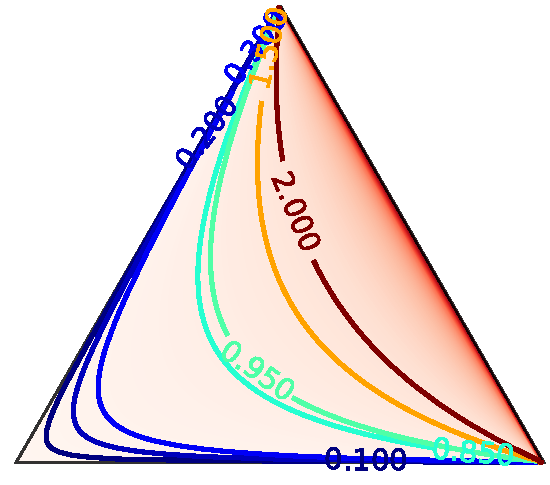
\includegraphics[height=2.14cm]{img/croppedDirichletGraph9.pdf}
        }\hspace{1in}
        \subfigure[\((1.5,1.5,1.5)\)]{
                \label{fig:subfig:d} %% label for third subfigure g
                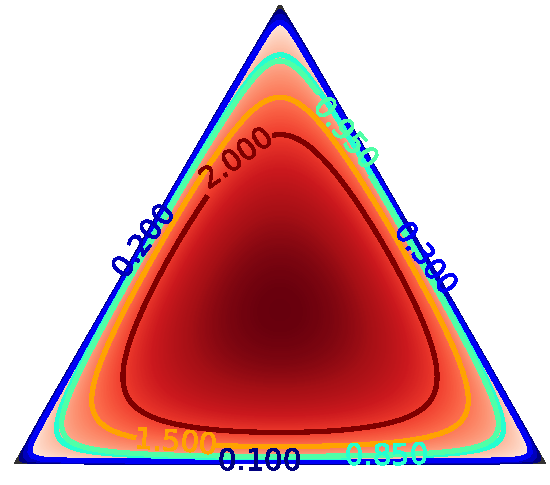
\includegraphics[height=2.14cm]{img/croppedDirichletGraph2.pdf}
        }
        \subfigure[\((2.5,2.5,2.5)\)]{
                \label{fig:subfig:a} %% label for first subfigure h
                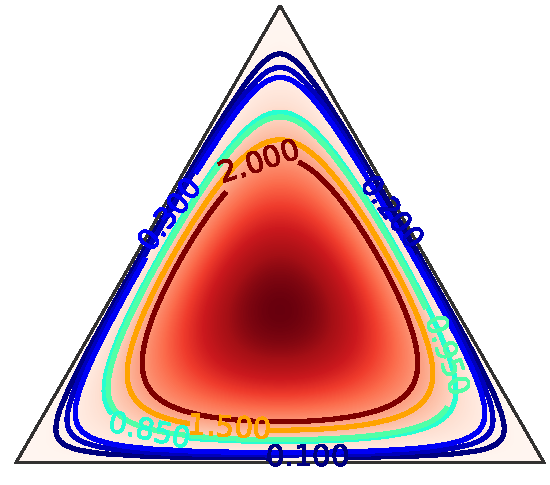
\includegraphics[height=2.14cm]{img/croppedDirichletGraph3.pdf}
        }
        \subfigure[\((1.5,1.5,2.5)\)]{
                \label{fig:subfig:d} %% label for third subfigure i
                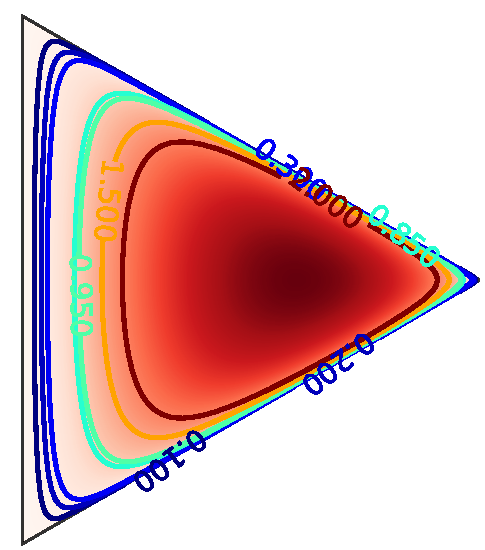
\includegraphics[height=2.14cm]{img/croppedDirichletGraph6.pdf}
        }
        \subfigure[\((2.5,2.5,3.5)\)]{
                \label{fig:subfig:d} %% label for third subfigure j
                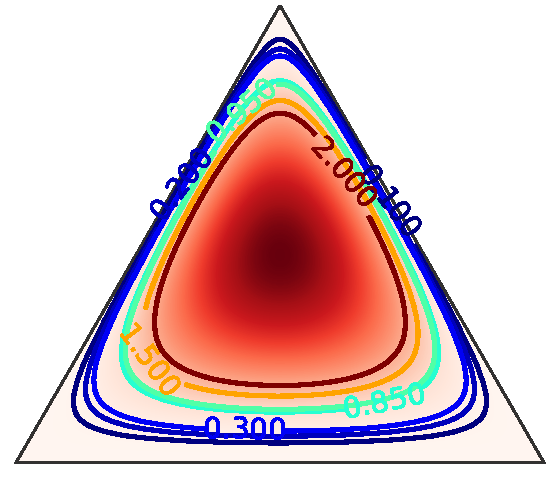
\includegraphics[height=2.14cm]{img/croppedDirichletGraph7.pdf}
        }
        \subfigure[\((1.5,2.5,2.5)\)]{
                \label{fig:subfig:d} %% label for third subfigure k
                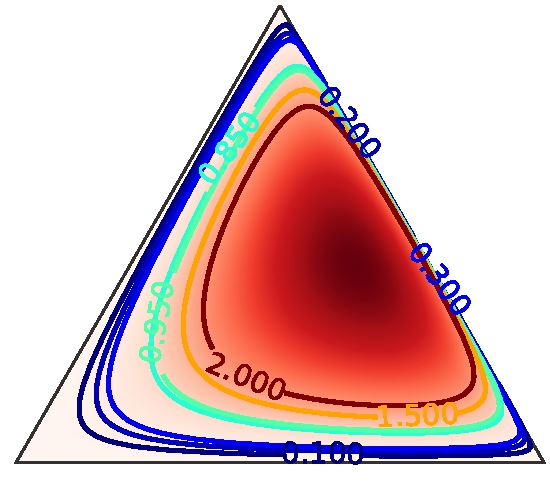
\includegraphics[height=2.14cm]{img/croppedDirichletGraph10.pdf}
        }
        \subfigure[\((2.5,3.5,3.5)\)]{
                \label{fig:subfig:a} %% label for first subfigure l
                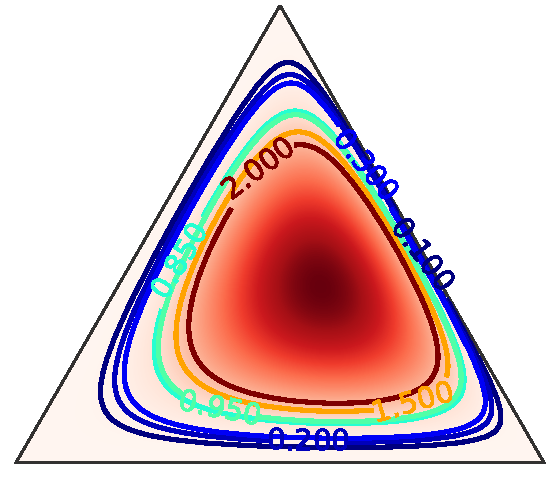
\includegraphics[height=2.14cm]{img/croppedDirichletGraph11.pdf}
        }\hspace{1in}
        \caption{Illustration of Dirichlet distribution's probabilistic density on the 3-dimensional simplex when given different priors. (a,b,g,h) the left four subfigures illustrate the probabilistic density when given the symetric priors for Dirichlet distribution; (c,d,i,j) the central subfigures illustrate the probablistic density given ; (e,f,k,l) }
\end{figure*}
\end{comment}


\section{Proposed Method}
Knowledge base often contains much information about what happened. 
But the existing RDF model\cite{klyne2006rdf} on knowledge base lacks an efficient mechanism to transfer the information from knowledge base to text stream.  
With the help of knowledge base's structure (detailed in sec \ref{subsec:hs_initialization}), we provide a  lightweight model to transfer the information in knowledge base to text stream.

\textit{History state} is the proposed data structure to restore the information about what happened. 
Initially, \textit{history state} extracts category-related history data into a set of tuples, which weighs the importance of given words to the specific category, defined in Definition 1 formally. 
Taking the \textit{military} category in Figure \ref{fig:modelDesc} as an example, the history state of \textit{military} contain the words \textit{army}, \textit{military}, and \textit{shootings} etc. 

\textit{Recent state} is the proposed data structure to maintain the information about what's happening.
It extracts category-related words from incoming text stream, for each time window.
Still taking the \textit{military} category in  Figure \ref{fig:modelDesc} as an example, based on extracted history states, our proposed probabilistic continuous learning model \textsc{HS-Prior-LDA} can recognize the words \textit{libyan} and \textit{rebel} in the time window 2011-07-28 in the text stream are related to the category \textit{military}. 
Furthermore the time series analysis on the neighbouring recent states can recognize the set of events' candidate words, and finally detects the events in the text stream. 
In the example of Figure \ref{fig:modelDesc}, the words \textit{libyan} and \textit{rebel} are related to the \textit{military} event ``\#libya Libyan rebels chief is killed (2011-07-28)''.

After processing each time window's data, the words in microblogs can be enriched semantically with knowledge base.
In this way, the transfer learning model provides richer semantics and less noise for microblog stream, which promotes the accuracy of event detection significantly. 
The following definitions are the concepts used by the transfer learning model \textsc{TransDetector}. 

\begin{rmk}[History State] 
The history state of the specific category is defined by a set of tuples, in which the first element is the word \(w^{(c)}_i\) related to the category \(c\), and the second element is the chi-square score \(chi(c,w^{(c)}_{i})\) under the category \(c\). 
And we denote the history states of category \(c\) as \(\bm{h}_c=\{<w^{(c)}_i,chi(c,w^{(c)}_{i})>\}_{i=1,...,N_c}\).
\end{rmk}

\begin{rmk}[Recent State] 
The recent state at time \(t\) of the specific category \(c\) is defined by a set of tuples, and denoted as \(\bm{r}_{c,t}=\{<w^{(c)}_i,n(c,t,w^{(c)}_{i})>\}_{i=1,...,N_c}\), in which word \(w^{(c)}_{i}\) is related to the category \(c\), and \(n(c,t,w^{(c)}_{i})\) is its document frequency in the time window \(t\).
\end{rmk}

\begin{rmk}[The Set of Events' Candidate Words] 
The set of events' candidate words \(\mathcal{B}_{c,t}\) are defined by the bursty words in recent state \(\bm{r}_{c,t}\).
\end{rmk}

\begin{rmk}[Event Phrase] 
Event phrase \(\mathcal{C}_{c,t,i}\) is the \(i\)-th combination of words which occurred in the set of events' candidate words \(\mathcal{B}_{c,t}\), and represents the \(i\)-th event happened in time \(t\) under the category \(c\).
\end{rmk}

\begin{rmk}[Event Related Microblogs] Event related microblogs \(\mathcal{D}_{c,t,i}\) are articles that relate to the \(i\)-th event in time \(t\) under the category \(c\), and correspond to the event phase \(\mathcal{C}_{c,t,i}\).
\end{rmk}


Section \ref{subsec:hs_initialization} explains the details of how to initialize history states from knowledge base.
Section \ref{subsec:rs_initialization} shows how to perform transfer learning for recent states.
And section \ref{subsec:detection} interprets the high accuracy event detection based on the processed recent states.
\begin{comment}
\begin{table}
\scriptsize
\caption{Notations used by \textsc{NSDetector}}
\label{tbl:notations}
\begin{tabular}{|c|p{0.06\columnwidth}|p{0.66\columnwidth}|} \hline
%first part: normalization initialization
\multirow{5}{0.13\columnwidth}{History States' Initialization} & \(G^{(0)}\) & Taxonomy's Graph in Knowledge Base\\ \cline{2-3}
& \(G^{(1)}\) & Category-Page Bipartite Graph in Knowledge Base\\ \cline{2-3}
& \(G^{(2)}\) & Page-Content Map in Knowledge Base\\ \cline{2-3}
& \(c\) & topic related category node in \(G^{(0)}\), \(G^{(1)}\) \\ \cline{2-3}
& \(K_{\bm{KB}}\) & number of pre-defined topics in Knowledge Base \\ \cline{2-3}
& \(h_{c,w}\) & word \(w\)'s history state (chi-square score) in category \(c\) \\ \hline
%second part: normalization maintenance
\multirow{4}{0.13\columnwidth}{Normal States Maintenance} & \(\lambda\) & normal state weight in  NS-Prior-LDA\\ \cline{2-3}
& \(\tau_{c,w}\) & word \(w\)'s prior knowledge confidence for topic \(c\) in NS-Prior-LDA\\ \cline{2-3}
& \(S_c\) & topic \(c\)'s all normal states related words \\ \cline{2-3}
& \(K\) & number of topics in NS-Prior-LDA such as \(K>K_{\bm{KB}}\)\\ \hline
%third part: event detection
\multirow{5}{0.13\columnwidth}{Event Detection} & \(\mathcal{B}_{c, t}\)  & event words set detected from topic \(c\) at time \(t\)  \\ \cline{2-3}
& \(\mathcal{G}_{c, t}\)  & hot word graph constructed from \(\mathcal{B}_{c, t}\) \\ \cline{2-3}
& \(\mathcal{C}_{c,t,i}\) & event \(i\)-th related words in topic \(c\) at time \(t\) \\ \cline{2-3}
& \(\mathcal{D}_{c,t,i}\) & event \(i\)-th related articles in topic \(c\) at time \(t\) \\ \cline{2-3}
& \(\rho\) & density threshold for the sub-graph constructed by event words  \\ \hline

\end{tabular}
\label{symbolsInModel}
\end{table}
\end{comment}


\subsection{History States' Extraction}\label{subsec:hs_initialization}
In this part, we discuss in detail how to initialize the history states from the given knowledge base. 
The knowledge base such as Wikipedia has the structure of classes, subclasses, instances, and the edges between them. 
This structure usually can be represented as triples in RDF graph\cite{klyne2006rdf}, which is adopted to build DBPedia\cite{auer2007dbpedia} and YAGO\cite{suchanek2007yago} from Wikipedia. 
But the reasoning and maintenance of knowledge on the graph is usually expensive\cite{broekstra2003inferencing,bursztyn2015reasoning}. 
To make a trade-off between cost and performance, we use the lightweight data structure \textit{history state} to represent the knowledge about what happened, which is extracted from the knowledge base.
And the knowledge base's threefold structure \(G^{(0)}\), \(G^{(1)}\), \(G^{(2)}\) benefits the extraction of history states. 

\textbf{Taxonomy Graph \(G^{(0)}\)}. The directed edges in \(G^{(0)}\) represent the \textit{class}\(\rightarrow\)\textit{subclass} relations in the knowledge base. 
Taking Wikipedia for example (Figure \ref{fig:NSinitializaton}), the node \textit{Main topic classifications}\footnote{\url{https://en.wikipedia.org/wiki/Category:Main_topic_classifications}} has the subclass \textit{Society}, further contains the subclass \textit{Politics}, which is the ancestor of the subclass \textit{Military}.
As \(G^{(0)}\) is not a Directed Acyclic Graph originally\cite{faralli2015large}, we remove the cycles according to nodes' PageRank-HITS\cite{Yan:2015wq} score.
Specifically, the edges \textit{class}\(\rightarrow\)\textit{subclass} are preserved only when the node \textit{class} has the higher PageRank-HITS score than the node \textit{subclass}, which is shown in the line \ref{alg:line2inNormalStatesInit} of Algorithm \ref{alg:normalStatesInit}.
After removing cycles, the taxonomy structure on the knowledge base is better represented by the directed acyclic graph \(G^{(0)'}\).
As shown in line \ref{alg:line3inNormalStatesInit} of Algorithm \ref{alg:normalStatesInit}, by visiting the category \textit{Military} in the DAG \(G^{(0)'}\), the breadth-first traverse can reach its successor sub-category nodes such as \textit{Firearms}, \textit{The World Wars}, and \textit{World War II}, etc. 

\textbf{Category-Page Bipartite Graph \(G^{(1)}\)}. 
The directed edges in \(G^{(1)}\) represent the \textit{class}\(\rightarrow\)\textit{instance} relations in the knowledge base.
In Wikipedia, by considering \(G^{(0)'}\) and \(G^{(1)}\) together as shown in line \ref{alg:line5inNormalStatesInit} of Algorithm \ref{alg:normalStatesInit}, we can get all the pages related to the given category. 

\textbf{Page-Content Map \(G^{(2)}\)}. 
For a specific Wikipedia dumps version, the edges  \textit{page} \(\rightarrow\)\textit{content} in \(G^{(2)}\) define a one-to-one mapping.
There are a bulk of history information restored in the wiki text content.
In order to extract the key words in wiki page's content, which distinguish it from other pages, we use the chi-square statistics\cite{yang1997comparative}\cite{liu2009imbalanced} to measure the importance of each word for the specific page.

For a given category in \(G^{(0)'}\), chi-square statistics also can evaluate the importance of each word appeared in text contents. 
For example, the chi-square statistic of the term \textit{shooting} under the category \textit{military} is 2888.7 under chi-square test with 1 degree of freedom.
That means the term \textit{shooting} is highly related to the category \textit{military}.  
%To prevent the overclaim of rare word by chi-square statitistcs, the word frequency is introduced as a supplement\cite{liu2009imbalanced}, as shown in line \ref{alg:line10inNormalStatesInit} of Algorithm \ref{alg:normalStatesInit}.
Finally, we can get the category's history state, which are  composed by the category related words and their corresponding importance.
%history states衡量一个词在考虑完整历史信息的情况下,对于一个类别的重要程度,例如在military类别下面;从某种程度上讲,history state从knowledge base中抽取了对于该类别的重要特征,有助于我们将它应用到text stream当中。
\setlength{\textfloatsep}{3pt}% Remove \textfloatsep
\begin{algorithm}[h]
\scriptsize
\caption{History State Initialization from Knowledge Base}
\label{alg:normalStatesInit}

\KwIn{Taxonomy's Graph \(G^{(0)}\), Category-Page Bipartite Graph \(G^{(1)}\), Page-Content Bipartite Graph \(G^{(2)}\), topic related category node \(c\)}
\KwOut{History state \(\bm{h}_c\) on category \(c\)}
\(Pages(c)\leftarrow \varnothing\), \(\bm{h}_c \leftarrow \varnothing\)\\
DAG \(G^{(0)'} \leftarrow\) Remove Cycles of \(G^{(0)}\) by nodes' HITS-PageRank scores. \label{alg:line2inNormalStatesInit}\\
\(SuccessorNodes(c) \leftarrow \) Breadth-first-traverse(\(G^{(0)'},c\))\label{alg:line3inNormalStatesInit}\\
\For{\(node \in SuccessorNodes(c)\)}{
    \(Pages(c) \leftarrow Pages(c) \cup G^{(1)}.neighbours(node)\) \label{alg:line5inNormalStatesInit}\\
}
Word frequency table \(n(c,.) \leftarrow \) do word count on the text contents of \(Pages(c)\) \\
Word frequency table \(n(All,.) \leftarrow \) do word count on the text contents of all pages in \(G^{(2)}\).\\
\For{word \(w\) in WordFrequencyTable(All).keys()}{
    \(chi(c,w) \leftarrow \) \(w\)'s chi-square statistics on \(WordFrequencyTable(c)\) and \(WordFrequencyTable(All)\).\\
    \(h_{c,w} \leftarrow chi(c,w)\) \label{alg:line10inNormalStatesInit}\\
}
\Return{\(\bm{h}_c\)}
\end{algorithm}

Considering the full Wikipedia's contents, history state evaluates the importance of word to the concerned category accurately. 
For example, in \textit{Military}'s history state, the top  words are \textit{army}, \textit{military}, \textit{air}, \textit{command}, \textit{force}, and \textit{regiment}, etc. 
The document which contains these words is related to the category \textit{Military} with high probability. 
We further discuss how to apply history states to the text stream on the following subsection \ref{subsec:rs_initialization}.

\subsection{Recent States' Maintenance}
\label{subsec:rs_initialization}
In this subsection, we describe how the proposed probabilistic model \textsc{HS-Prior-LDA} utilizes the history states to learn the recent states from text stream.

There are two facts inspiring \textsc{HS-Prior-LDA}. 
(1) The topics in the document may contain history-state-like topics. 
As an example, the tweet ``Libyan rebel chief gunned down in Benghazi (2011-07-28)'' contains the topic that is similar to the \textit{Military}'s history state.
(2) The history-state-like topics can reuse the information  stored in the history states.
The word \textit{libyan} in the aforementioned example tweet ranks much higher in the \textit{Military} and the \textit{Middle East} history states than the other categories' history states.
After considering the relatedness between the remaining context and the history states, the learned topics of the example tweet include \textit{Military} and \textit{Middle East}. 

The generative process of \textsc{HS-Prior-LDA} can be described as follows.

\begin{enumerate}[itemsep=0mm]
\item Draw corpus prior distribution \(\bm{m} \sim Dir(\alpha \bm{u})\), where \(\bm{u}\) is the uniform distribution.
\item For each topic \(k \in \{1,\cdots,K\}\), 
\begin{enumerate}[itemsep=0mm]
\item word distribution on the topic \(\bm{\phi_k} \sim Dir(\bm{\beta}+ \bm{\tau_k})\).
\end{enumerate}
\item For each document index \(d \in \{1,\cdots,D\}\),
\begin{enumerate}[itemsep=0mm]
\item topic distribution on the document \(\theta_d \sim Dir(\bm{m})\),
\item for each word index \(n \in \{1,\cdots,N_d\}\),
\begin{enumerate}[itemsep=0mm]
\item word's topic assignment \(z_{dn} \sim Multinomial(\theta_d)\), 
\item word \(w_{dn} \sim Multinomial(\phi_{z_{dn}})\). 
\end{enumerate}
\end{enumerate}

\end{enumerate}

In the above generative process, the line 2(a) is the key point to distinguish \textsc{HS-Prior-LDA} from LDA\cite{blei2003latent}, where \(\bm{\tau}_k\) is defined by Equation(\ref{eq:wikiPrior}).
\(K_{KB}\) is the number of pre-defined history-state-like topics, and \(S_k\) is the set of words appeared in the \(k\)-th topic's history state.
As \cite{wallach2008structured} mentioned that the asymmetric prior distribution can significantly improve the quality of topic modelling, \(\bm{\phi_k} \sim Dir(\bm{\beta}+ \bm{\tau_k})\) incorporates history state into the asymmetric prior of the word distribution on topic. 
The effect of \(\bm{\tau_k}\) is obvious, e.g., \(\tau_{Military,army}/\tau_{Military,basketball}=203\) leads to that topic \textit{Military} prefers to contain the word \textit{army} other than \textit{basketball}.
The parameter \(\lambda\) controls how much the learned topics are similar to the history state, which can be chosen by cross-validated grid-search. 

\begin{scriptsize}
\begin{equation}
\label{eq:wikiPrior}
\begin{aligned}
\tau_{kv}=
\left\{ \begin{aligned}
\lambda \frac{h_{kv}}{\sum_{v\in S_{k}}h_{kv}} &,v\in S_{k}\ and  \ k \leq K_{\bm{KB}} \\
0&,v \notin S_{k} \ or \ k > K_{\bm{KB}} \\
\end{aligned}\right.
\end{aligned}
\end{equation}
\end{scriptsize}

\begin{comment}
\begin{figure}[t]
    \centering
    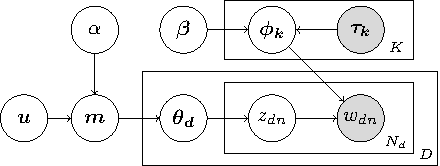
\includegraphics[width=0.75\columnwidth]{model/lda_tikz.pdf}
    \caption{Probabilistic model for training normal states by using history information.}
    %The convolution neural network for extracting character-level representations of words. Dashed arrows indicate a dropout layer applied before character embeddings are input to CNN.}
    \label{fig:NS-Prior-LDA}
\end{figure}
\end{comment}

To solve \textsc{HS-Prior-LDA}, the gibbs sampling is adopted to determine the hidden variable \(z_{dn}\) and the model parameter \(\phi_k\).
In the initialization phase of Gibbs sampling for \textsc{HS-Prior-LDA}, the hidden variable \(z_{dn}\) is initialized to topic \(k\) with probability \(\hat{q}_{k|v}\) as Equation (\ref{eq:initProbability}).
For the word \(v\) that belongs to any history state, \(\hat{q}_{k|v}\) is proportional to its importance in the history state \(\tau_{kv}\) as Eq\ref{eq:initProbability}(a). 
For the new word \(v\) in text stream, \(\hat{q}_{k|v}\) is   set uniformly \(1/(K-K_{\bm{KB}})\) on the other topics as Eq\ref{eq:initProbability}(b,c). 
The initialization makes sure that the learned topics are aligned to the pre-defined history states.
\begin{scriptsize} 
\begin{equation}
\label{eq:initProbability}
\begin{aligned}
\hat{q}_{k|v}=
\left\{ \begin{aligned}
\frac{\tau_{kv}}{\sum_{k=1}^{K}\tau_{kv}} &,\sum_{k}\tau_{kv}>0 & (a)\\
0&, \sum_{k}\tau_{kv}=0 \ and \ k \leq K_{\bm{KB}} & (b)\\
1/(K-K_{\bm{KB}})&,\sum_{k}\tau_{kv}=0 \ and \ k > K_{\bm{KB}} & (c)
\end{aligned}\right.
\end{aligned}
\end{equation}
\end{scriptsize}

%采样公式p(z|.),z有两部分。
The sampling process uses the conditional probability \(p(z_{dn}=k|.)\propto (n^{(d)}_{dk}+\alpha m_k)(n^{(w)}_{kv}+\tau_{kv}+\beta)/(n^{(w)}_{k,.}+\tau_{k,.}+V\beta)\), where \(n^{(d)}_{dk}\) is the number of words in document \(d\) assigned to topic \(k\), and \(n^{(w)}_{kv}\) is the times of word \(v\) assigned to topic \(k\).
We also optimize \(\alpha \bm{m}\) for promoting \textsc{HS-Prior-LDA}'s fitting to documents according to \cite{wallach2008structured}\footnote{\url{https://github.com/mimno/Mallet/blob/master/src/cc/mallet/types/Dirichlet.java}}.\begin{comment}
\begin{equation}
\label{eq:KBPriorLDAgibbs}
\begin{aligned}
&p(z_{dn}=k|w_{dn}=v,z_{\neg{dn}},w_{\neg{dn}},\alpha\bm{m},\beta,\tau)\\
&\ \ \propto (n^{(d)}_{dk}+\alpha m_k)\frac{n^{(w)}_{kv}+\tau_{kv}+\beta}{n^{(w)}_{k,.}+\tau_{k,.}+V\beta}
\end{aligned}
\end{equation}
\end{comment}

\begin{comment}
\begin{scriptsize}
\begin{equation}
\label{eq:KBPriorLDAgibbs}
\begin{aligned}
&p(z_{dn}=k|w_{dn}=v,z_{\neg{dn}},w_{\neg{dn}},\alpha\bm{m},\beta,\tau)\\
&\ \ \propto (n^{(d)}_{dk}+\alpha m_k)\frac{n^{(w)}_{kv}+\tau_{kv}+\beta}{n^{(w)}_{k,.}+\tau_{k,.}+V\beta}
\end{aligned}
\end{equation}
\end{scriptsize}
\end{comment}

\begin{comment}
\begin{algorithm}
\scriptsize
\caption{NS-Prior-LDA Learning Algorithm}
\label{alg:gibbsSamplingKBPriorLDA}
\KwIn{Documents \(\mathcal{D}\) (a.k.a., \(\bm{w_{1:D}}\)), and normal states \(\bm{f}_{1:K_{\bm{KB}}}\)}
\KwOut{The sufficient statistics \(\bm{n^{(d)}}\), \(\bm{n^{(w)}}\)}
\tcc{Initialization of NS-Prior-LDA}
\For{\(d=1:D\)}{
    \For{\(n=1:N_d\)}{
        \(v=w_{dn}\), sample \(z_{dn}=k\) as Eq(\ref{eq:wikiPrior})(\ref{eq:initProbability}).\\
        Update the sufficient statistics \(n^{(d)}_{d,k}\), \(n^{(w)}_{k,v}\).\\
            }
        }
\For{\(i= 1:I\)}{
    \tcc{E-Step of NS-Prior-LDA}
    \For{\(i=1:I_E\)}{
        \For{\(d=1:D\)}{
            \For{\(n=1:N_d\)}{
                Set \(v=w_{dn}\), and reset the sufficient statistics \(n^{(d)}_{d,z_{dn}}\), \(n^{(w)}_{z_{dn},v}\).\\
                Resample \(z_{dn}=k\) as Eq(\ref{eq:wikiPrior})(\ref{eq:KBPriorLDAgibbs}).\\
                Update the sufficient statistics \(n^{(d)}_{d,k}\), \(n^{(w)}_{k,v}\).\\
            }
        }
    }
    \tcc{M-Step of NS-Prior-LDA}
    Optimize \(\alpha \bm{m}\) by the fixed-point iteration\cite{wallach2008structured}. 
}
\Return{\(\bm{n^{(w)}}\)}
\end{algorithm}
\end{comment}

After Gibbs sampling on discrete time windows, \textsc{HS-Prior-LDA} learned all hidden topics of words in microblog stream.
And for a specific word type \(w\) and its history-state-like topic assignment \(c\) in time window \(t\), its document frequency is counted as \(n(c,t,w^{(c)})\), which is the element of category \(c\)'s \(t\)-th recent state.
Event detection on recent states is discussed in the following subsection.

\subsection{Detecting Events from Recent States}
\label{subsec:detection}
After transfer learning, events are detected accurately because the word time series is refined to finer grain as multiple corresponding (word, category) time series, and the bursty pattern is better exposed. 
Taking the word \textit{hood} as an example, it belongs to the category \textit{Military} when it appeared in \textit{Ft Hood}, a US military establishment located in Texas.
As shown in Figure \ref{fig:hood}, the bursty pattern of \textit{hood} is clearly exposed after distinguishing its \textit{Military} time series from the raw one.
%Therefore, the processing on each category's accurate stream states leads to the accurate event detection. 

Given (word, category) time series and microblogs in a time window, we take the detection in	 three sub-phases: (1) detecting events' candidate words; (2) generating event phrases; (3) retrieving event related microblogs.
Note that these sub-phases are also available for the common text stream, but they performs better when words are enriched by category concepts of knowledge base.
%这里添加对这几个Definition的解释。

\textbf{Detecting events' candidate words}. For a word \(w\) and a category \(c\), on its time series \(\{n(c,t,w^{(c)})\}_{t=1}^{T}\), many bursty detection methods can be applied to check if the word \(w\) is bursty in category \(c\) by given time \(t\). 
We assume the document frequency of \(w^{(c)}\) follows a poisson distribution, which is also used in \cite{Diao:2012wj}.
And the document frequency of nonbursting \(w^{(c)}\) has the possison distribution with the parameter \(\lambda=\mu_0\); while the bursting one with the parameter \(4\mu_0\) means the document frequency \(n(c,t,w^{(c)})\) is much higher when bursting.
We empirically set \(\mu_0\) as the moving average \(\mu_0^{(t)}=\frac{1}{T}\sum_{\tau=t-T}^{t-1}n(c,\tau,w^{(c)})\), and set T=10.
Hence, at time \(t\), bursty or not is determined by comparing the probabilities of above poisson distributions. 
After bursty detection on the time series, we add each time \(t\)'s bursty word \(w^{(c)}\) into the set of event's candidate words \(\mathcal{B}_{c,t}\).

\textbf{Generating event phrases}. 
In the set of event's candidate words \(\mathcal{B}_{c,t}\), some words appear together and should be grouped into event phrases.
For example, there are six bursty words in \(\mathcal{B}_{military,2011-07-28}\) belonging to two event phrases \textit{``ft, hood, attack"} and \textit{``libyan, rebel, gunned"} in the time window 2011-07-28 to represent the events happened to the US military establishment and the Libyan rebel respectively. 

In order to group the bursty words together, we  construct the directed weighted graph \(\mathcal{G}_{c,t}=(\mathcal{B}_{c,t},\mathcal{E}_{c,t},\mathcal{W}_{c,t})\), where \(\mathcal{E}_{c,t}=\{(a,b)|a \in \mathcal{B}_{c,t}, b \in \mathcal{B}_{c,t}, PMI(a,b)>0 \}\), and \(\mathcal{W}_{c,t}\) gives the PMI scores on the edges.
The graph \(\mathcal{G}_{c,t}\) means the words in \(\mathcal{B}_{c,t}\) are connected if and only if their PMI score in the given time window's microblogs is over 0. 

Given the graph \(\mathcal{G}_{c,t}\), spectral clustering\cite{von2007tutorial} is utilized for exploring the best partition of words. 
To get the optimum cluster number, we use the graph density as the criteria.
The graph density is the ratio of the number of edges to that of complete graph (the graph with all possible edges), and in practice all the sub-graphs in \(\mathcal{G}_{c,t}\) should have the densities over an empirical threshold. 
And the empirical threshold is set to 0.6 in our setting.
We run the spectral clustering with cluster number from 1 to \(|\mathcal{B}_{c,t}|\), and stop when all the resulting sub-graphs satisfy the criteria that the density is over the given threshold. 
In this way, the generated event phrase combines the co-occurred bursty words and excludes the unrelated. 


\textbf{Retrieving event related microblogs}. 
To better understand the event, we retrieve the event microblogs \(\mathcal{D}_{c,t,i}\) by using the event phrase \(\mathcal{C}_{c,t,i}\).
Generally, according to the number of bursting words in the event phrase \(\mathcal{C}_{c,t,i}\), there are two situations to be addressed. 
(1) \(|\mathcal{C}_{c,t,i}|=1\), we directly add the microblog in time window \(t\), which contains the bursting category-word \(w^{(c)}\), into the set \(\mathcal{D}_{c,t,i}\).
(2) \(|\mathcal{C}_{c,t,i}|\geq 2\), it's not necessary that all the bursting words are included in the event related microblog.
For example, the tweet ``\textit{Soldier wanted to attack Fort Hood troops}" contains the bursting words \textit{attack} and \textit{hood}, not all the event phrase ``\textit{ft, hood, attack}". 
To tackle this problem, we consider the microblog, that contains any pair of category-words in the event phrase, as the event related microblog.

Finally, \textsc{TransDetector} gets the detected events \(\{(\mathcal{C}_{c,t,i},\mathcal{D}_{c,t,i})\}_{i=1}^{|\mathcal{C}_{c,t}|}\), containing the event phrase and the corresponding event related microblogs for the given category and the time window.

%Text stream evolves more quickly with time than knowledge base.
%For example, recent state of Military contain .
%In other words, recent state is history-state-like topic timestamp.%在时间轴上的横截面。





\section{Experiments}
\subsection{Data Sets}
In this subsection, we demonstrate the effectiveness of \textit{history states} initialized from knowledge base and \textit{recent states} learned by transfer learning. 

\textbf{Knowledge Base.} 
We construct the taxonomy graph \(G^{(0)}\), the category-page bipartite graph \(G^{(1)}\) from the latest dump of category links\footnote{\url{https://dumps.wikimedia.org/enwiki/latest/enwiki-latest-categorylinks.sql.gz}} and the page-content map \(G^{(2)}\) from Wikipedia pages\footnote{\url{https://dumps.wikimedia.org/enwiki/latest/enwiki-latest-pages-articles.xml.bz2 }}.
We set \(K_{KB}=100\), which means 100 categories are selected manually to cover the topics of Wikipedia and the target corpus as widely as possible. 
There are two kinds of categories are considered. 
The mid-high categories in the taxonomy graph \(G^{(0)'}\), which are representative, are likely to be selected, such as \textit{Aviation}, \textit{Military}, and \textit{Middle East}, etc.
And the mid categories, which reflect the main interests of the target corpus, are also taken into consideration, such as \textit{American Football}, \textit{Basketball}, and \textit{Baseball}, etc. 
%Other knowledge bases which have the above mentioned threefold structure are also available for conducting.

\textbf{Microblog Stream Dataset.} We conduct the empirical analysis on a text stream benchmark \textit{Edinburgh twitter corpus} which is constructed by \cite{petrovic2012using} and widely used by previous event detection researches \cite{petrovic2013can} \cite{Wurzer:2015wq}. 
Due to the developer policy of Twitter, \cite{petrovic2012using} only redistributes tweets' IDs\footnote{\url{http://demeter.inf.ed.ac.uk/cross/docs/fsd_corpus.tar.gz}}.
%\footnote{\url{https://dev.twitter.com/overview/terms/policy}}
We collected the tweets' contents according to the IDs with the help of Twitter API. 
Though we cannot get the whole dataset due to the limit of Twitter API, after necessary pre-processing, our rebuilt dataset still contains 36,627,434 tweets, which spans identically from 2011/06/30 to 2011/09/15.
More details of the original dataset are described in \cite{petrovic2010edinburgh}.

\subsection{Effects of Categroy-Level Topics}
The category-level topics are initialized on the pre-defined categories from the knowledge base as Algorithm \ref{alg:normalStatesInit}.
%This process is illustrated by Table \ref{tbl:historyStates}. 

\textbf{Evaluation Metrics.}
We compare the topic coherence of history states with the topics learned from Wikipedia by LDA in terms of NPMI\cite{Rder2015ExploringTS}.
Different from traditional experiments that only compute the topic coherence of top words, we want to check whether  it can hold for more words.
Due to the limit of NPMI computing module\footnote{\url{https://github.com/AKSW/Palmetto}}, which computes the coherence of up to 10 words each time, we compute NPMI on the combination of top five words with each next five words as Table \ref{tbl:NPMIDetails}.

\textbf{Results.}
Observe that even for the combination of 96th to 100th words with the top five words in \textit{Aviation}'s history state, NPMI=0.131 shows that the topic coherence still holds well without drifting.
More generally, Figure \ref{fig:NPMI} illustrates that the history states are much more stable than the topics learned by LDA.
Taking the group 10 (the combination of 56th to 60th words with the top five words) as an example, the median one of history states performs better than all those learned by LDA. 

Since the history states extracted from knowledge base is stable and topic coherence, 

%\hlgreen{TODO: add a new table, containing a topic generated by BTM, which is most similar to the extracted topic from KB.}
\begin{table}[h]
\setlength{\abovecaptionskip}{0.cm}%set the distance between caption and table to 0 cm.
\setlength{\belowcaptionskip}{0.cm}
\centering
\caption{Top words' topic coherence of \textit{Aviation}'s history state. * means the group also contains the five top words \textit{aircraft}, \textit{air}, \textit{airport}, \textit{flight}, and \textit{airline}, but we don't show them in table to save space. NPMI is computed on ten words (a combination of words in each row with the five top words).}
\scalebox{0.65}{
\begin{tabular}{|c|l|l|l !{\vrule width 1pt} c|l|l|l|}
\hline
\multicolumn{4}{|c!{\vrule width 1pt}}{Category-Level Topics extracted from Wikipedia by \textsc{TransDetector}} & \multicolumn{4}{c|}{Topics Learned from Wikipedia by LightLDA}    \\ \hline
Group ID& \#words*  & words  & NPMI & Group ID& \#words*& words & NPMI \\ \hline
-1 & 1-5 & aircraft air airport flight airline &  & -1 & 1-5 & engine aircraft car air power & \\ \hline
0 & 6-10 & airlines aviation flying pilot squadron &  0.113 & 0 & 6-10 & design flight model production speed & 0.112\\ \hline
1 & 11-15 &flights pilots raf airways fighter & 0.155 & 1 & 11-15 &system vehicle cars engines mm & 0.062\\ \hline
2 & 16-20 &boeing runway force crashed flew   & 0.092 & 2 & 16-20 & fuel vehicles designed models type & 0.072\\ \hline
3 & 21-25 &airfield landing passengers plane aerial & 0.179 & 3 & 21-25 & version front produced rear electric & 0.035\\ \hline
4 & 26-30 &bomber radar wing bombers crash & 0.137 & 4 & 26-30 & space control motor standard development & 0.085\\ \hline
5 & 31-35 &airbus airports operations jet helicopter & 0.189 & 5 & 31-35 & film range light using available & -0.002\\ \hline
6 & 36-40 &squadrons base flown havilland crew & 0.088 & 6 & 36-40 & wing powered wheel weight launch & 0.087\\ \hline
7 & 41-45 &combat luftwaffe aerodrome carrier fokker & 0.159 & 7 & 41-45 & developed low test ford cylinder & 0.007\\ \hline
8 & 46-50 &planes fly engine takeoff fleet & 0.186 & 8 & 46-50 & equipment side pilot hp aviation & 0.091\\ \hline
9 & 51-55 &fuselage helicopters aviator naval aero & 0.157 & 9 & 51-55 & systems us sold body drive & -0.051\\ \hline
10 & 56-60 &glider command training balloon faa & 0.166 & 10 & 56-60 & gear introduced class safety seat & 0.069\\ \hline
\(\cdots\) & \(\cdots\) &\(\cdots\) &\(\cdots\) & \(\cdots\) & \(\cdots\) &\(\cdots\) &\(\cdots\)\\ \hline
18 & 96-100 &scheduled carriers military curtiss biplane &0.131 & 18 & 96-100 & transmission special replaced limited different & 0.059\\ \hline
19 & 101-105 &accident engines iaf albatross rcaf &0.068 & 19 & 101-105 & features machine nuclear even unit & 0.011\\ \hline
\end{tabular}
}
\label{tbl:NPMIDetails}
\end{table}

\begin{figure}[h]
	\setlength{\abovecaptionskip}{0.cm}
	\setlength{\belowcaptionskip}{0.cm}
        \centering
        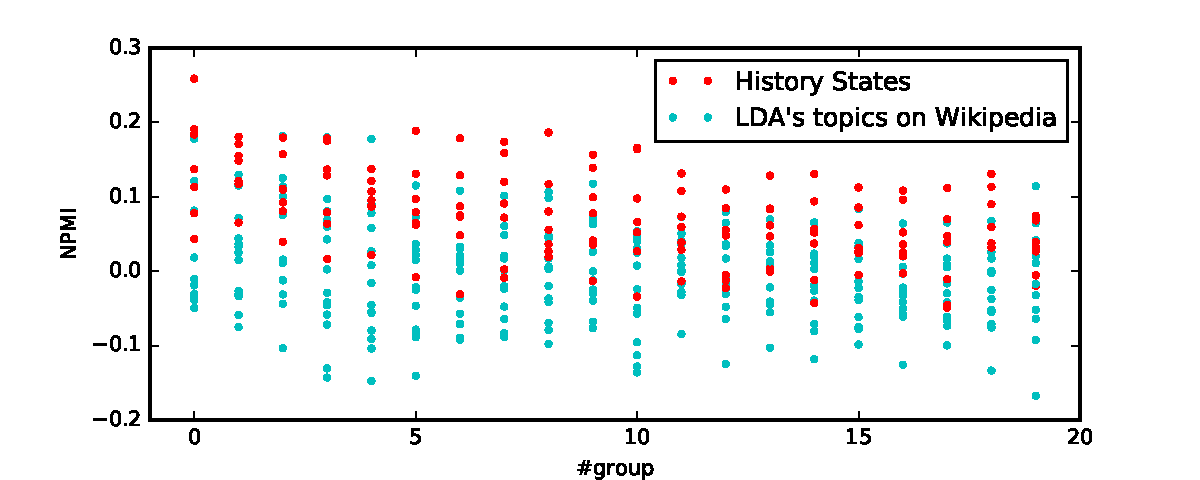
\includegraphics[width=1.0\columnwidth]{img/NPMI.pdf}
        \caption{The variable that has the greatest impact on the outcome is its newsworthiness.}
        \label{fig:NPMI}
\end{figure}

\textbf{Category-Level Topics Learned from Microblog Stream.}
For Trans-LDA, \(K\) is set to be 200, which means Trans-LDA learned 100 history-state-like topics and 100 other topics.
After cross-validated grid-search, \(\lambda\) is set to be 12.8. The other parameters are set as \(\alpha=0.1\), \(\beta=0.005\).
We run \textsc{Trans-LDA} window by window on text stream, and learn specific categories' topics.




%如图(topic)中,能够从Military*中学习出tweet(20110728)话题中包含libyan。


%We use 20newsgroups\cite{lang1995newsweeder} dataset\footnote{\url{http://qwone.com/~jason/20Newsgroups}} to check the effects of normal states initialization.

\begin{comment}
\begin{table}[]
\tiny
\centering
\caption{Normal State's cateogries corresponding to the 20-newsgroups corpus, and the F1 score on the classification task}
\label{my-label}
\begin{tabular}{|l|l|l|l|l|}
\hline
 &  & LDA & BOW  & \begin{tabular}[c]{@{}l@{}}NS-Prior-\\ LDA\end{tabular} \\ \hline
comp.graphics & Computer graphics &  &  &    \\ \hline
comp.os.ms-windows.misc & Microsoft Windows &  &  &    \\ \hline
comp.sys.ibm.pc.hardware & IBM personal computers &  &  &    \\ \hline
comp.sys.mac.hardware & Macintosh computers &  &  &    \\ \hline
comp.windows.x & X Window System &  &  &    \\ \hline
rec.autos & Automobiles &  &  &    \\ \hline
rec.motorcycles & Motorcycles &  &  &    \\ \hline
rec.sport.baseball & Baseball &  &  &    \\ \hline
rec.sport.hockey & Hockey &  &  &    \\ \hline
sci.crypt & Cryptography &  &  &    \\ \hline
sci.electronics & Electronics &  &  &    \\ \hline
sci.med & Medicine &  &  &    \\ \hline
sci.space & Outer space &  &  &    \\ \hline
misc.forsale & Sales &  &  &    \\ \hline
talk.politics.misc & Politics &  &  &    \\ \hline
talk.politics.guns & Gun politics &  &  &    \\ \hline
talk.politics.mideast & Middle East &  &  &   \\ \hline
talk.religion.misc & Religion &  &  &    \\ \hline
alt.atheism & Atheism &  &  &    \\ \hline
soc.religion.christian & Christians &  &   &  \\ \hline
In total &  &  &  & \\ \hline
\end{tabular}
\end{table}
\end{comment}

\begin{comment}
\begin{figure}
        \centering
        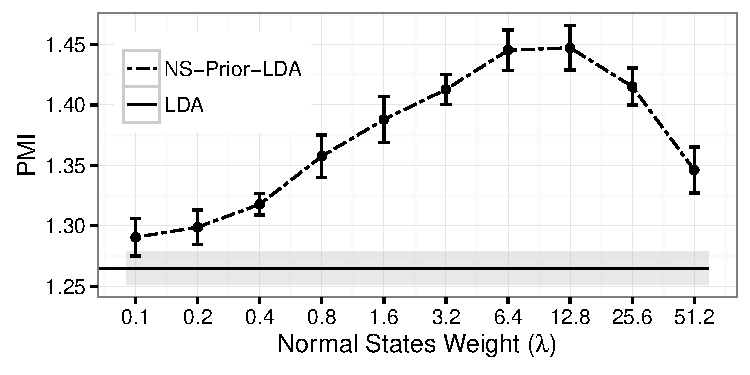
\includegraphics[height=4.0cm]{img/pmi.pdf}
        \caption{The quality of all twitter topics learned by NS-Prior-LDA increases with normal states weight (\(\lambda\)) before \(\lambda=12.8\). The optimized PMI is gained with moderate normal states weight when considering topics \(k\leq K_{\bm{KB}}\) and topics \(k > K_{\bm{KB}}\) together.}
\end{figure}
\end{comment}

\begin{comment}
\begin{table}
\centering
\caption{The PMI of twitter topics learned by NS-Prior-LDA, its variant, and other baselines}
    \begin{tabular}{|l|l|c|}
    \hline
    Model & Prior Knowledge & PMI \\ \hline
    LDA & None  & 1.265 \(\pm\) 0.013     \\ \hline
    BurstyBTM\cite{Yan:2015wm} & None    & 1.467 \(\pm\) 0.017     \\ \hline
    NS-Prior-LDA\(^{(-)}\)   &   \begin{tabular}[c]{@{}l@{}}\footnotesize{Words in categories simply}\\ \footnotesize{extracted from Wikipedia}\end{tabular} & 1.439 \(\pm\) 0.010     \\ \hline
    NS-Prior-LDA         & \begin{tabular}[c]{@{}l@{}}\footnotesize{Normal states initialized} \\\footnotesize{from wikipedia}\end{tabular} & 1.523 \(\pm\) 0.017     \\ \hline
    \end{tabular}
\label{tbl:NS-Prior-LDA}
\end{table}
\end{comment}

\begin{table*}[ht]
\setlength{\abovecaptionskip}{0.cm}%set the distance between caption and table to 0 cm.
\setlength{\belowcaptionskip}{0.cm}
\centering
\caption{Category-Level Topics extracted from knowledge base and the corresponding topics on microblog stream learned from Trans-LDA, taking the categories \textit{Aviation},  \textit{Health}, \textit{Middle East}, \textit{Military}, and \textit{Mobile Phones} as examples. The words in \textbf{\textit{bold italic}} font are newly learned on the microblog stream by the transfer learning, which semantic meanings are verified consistent with the categories; while the words in normal font play the role as the bridge in transfer learning, and appear in the both category-level topics in two domains.}
\scalebox{0.8}{
\begin{tabular}{|cc|cc|cc|cc|cc|cc|}
\hline
\multicolumn{2}{|c|}{\textit{Aviation}} & \multicolumn{2}{c|}{\textit{Health}} & \multicolumn{2}{c|}{\textit{Middle East}} & \multicolumn{2}{c|}{\textit{Military}} & \multicolumn{2}{c|}{\textit{Mobile Phones}}\\
\begin{tabular}[c]{@{}c@{}}Knowledge\\ Base\end{tabular} & \begin{tabular}[c]{@{}c@{}}Microblog\\ Stream\end{tabular} & \begin{tabular}[c]{@{}c@{}}Knowledge\\ Base\end{tabular} & \begin{tabular}[c]{@{}c@{}}Microblog\\ Stream\end{tabular} & \begin{tabular}[c]{@{}c@{}}Knowledge\\ Base\end{tabular} & \begin{tabular}[c]{@{}c@{}}Microblog\\ Stream\end{tabular} & \begin{tabular}[c]{@{}c@{}}Knowledge\\ Base\end{tabular} & \begin{tabular}[c]{@{}c@{}}Microblog\\ Stream\end{tabular} & \begin{tabular}[c]{@{}c@{}}Knowledge\\ Base\end{tabular} & \begin{tabular}[c]{@{}c@{}}Microblog\\ Stream\end{tabular} \\ 
\hline
aircraft & air & health & weight & al & \textbf{\textit{\#syria}} & army & killed & android & iphone\\ 
air & plane & patients & loss & israel & \textbf{\textit{\#bahrain}} & military & news & mobile & apple \\ 
airport & flight & medical & diet & iran & people & air & \textbf{\textit{\#libya}} & nokia & android \\ 
flight & time & disease & health & arab & israel & command & libya & ios & app \\
airline & airlines & treatment & cancer & israeli & police & force & rebels & phone & ipad \\
airlines & news & hospital & lose & egypt & \textbf{\textit{\#libya}} & regiment & people & samsung & samsung \\
aviation & boat & patient & fat & egyptian & \#egypt & forces & police & game & mobile\\
flying & airport & clinical & tips & ibn & news & squadron & war & app & blackberry \\
pilot & force & symptoms & treatment & jerusalem & \textbf{\textit{\#israel}} & infantry & libyan & iphone & tablet \\
squadron & fly & cancer & body & syria & world & battle & attack & htc & apps\\
\hline
\end{tabular}
}
\label{tbl:historyStates}
\end{table*}
%TODO: add the top words in the category-level topic 
%\hlgreen{TODO: add the top words of the category-level topic in each window of microblog stream AFTER Table 2.}

%TODO: add the effect of transfer learning by using text classification, compared with fastText and SVM.
%\hlgreen{TODO: add the effect of transfer learning by using text classification, compared with fastText and SVM.}
\begin{comment}
\begin{figure*}
    \label{fig:algorithm}
    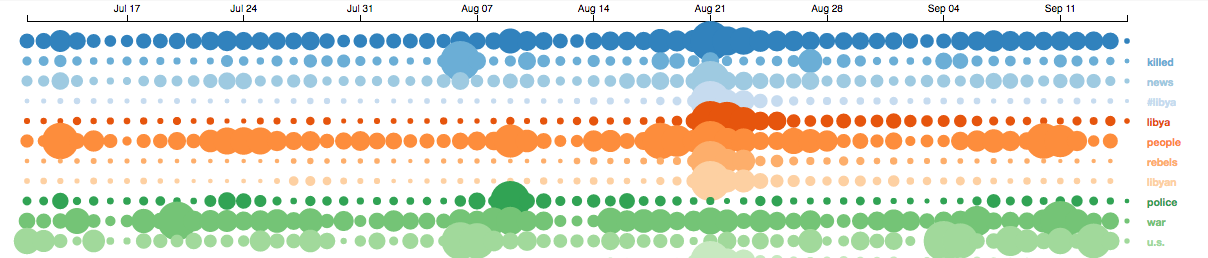
\includegraphics[width=1.0\textwidth]{img/screenShot.png}
    \caption{An illustration of the time series of Military related states on Twitter dataset from 2011-06-30 to 2011-09-15.}
\end{figure*}
\end{comment}

\subsection{Effects of Event Detection}
\textbf{Baselines Methods.} We compare our proposed method against the following methods, Twevent\cite{Twevent2012}, BurstyBTM\cite{Yan:2015wm}, LSH\cite{Petrovic:2010uj}, EDCoW\cite{Weng:2011wz}, and TimeUserLDA\cite{Diao:2012wj}, which are mentioned in the Section \ref{sec:relatedWorks}.
We implement these competing methods based on the open source community versions, e.g. EDCoW\footnote{\url{https://github.com/Falitokiniaina/EDCoW}}, or the authors' releases, e.g. BurstyBTM\footnote{\url{https://github.com/xiaohuiyan/BurstyBTM}}.
The above methods are set carefully according to the descriptions in the papers.
More precisely, (1) for LSH, 13 bits per hash table, 20 hash tables are set, and top 500 clusters with high entropy are selected as the event candidates; (2) for Twevent, the number of candidate bursty segments is set to be the square root of the window size, the newsworthiness threshold is set to be 4, and 375 candidate events are detected; (3) for EDCoW, the tunable parameter \(\gamma\) value is set to be 40, and 192 bursty ``phrases" are found for evaluation; (4) for TimeUserLDA, the topic number is set to be 500, and the most 100 bursty topics are selected as candidate events; (5) for BurstyBTM, the topic number is set to be 200, which is also the number of bursty topics in the model.
The information about the number of events to be evaluated is listed in Table \ref{tbl:overall}, where TransDetector detects 457 events after filtering out too niche events that contain less than 20 tweets. 

\textbf{Benchmarks and Evaluation Metrics.} 
The evaluation is conducted on two benchmarks.
The first benchmark on \textit{Edinburgh twitter corpus} contains 27 manually labeled events\cite{petrovic2013can}\footnote{\url{http://demeter.inf.ed.ac.uk/cross/docs/Newswire_Events.tar.gz}}, which all exist in our rebuilt dataset on the \textit{Edinburgh twitter}'s IDs.
These labeled events focus on the events that are both mentioned in twitter and newswire,e.g. \textit{``Oslo Attacks"} and \textit{``US Increasing Debt Ceiling"}, but still miss many important events such as \textit{``Hurricane Irene"}, \textit{``Al-Qaida's No. 2 Leader Being Killed"}, and popular events such as \textit{``Harry Potter and the Deathly Hallows (Part 2)"}.
To include these important events and enlarge the ground truth of realistic events pool, we build the second benchmark carefully.
We manually evaluate the candidate events detected by LSH,  \textsc{TransDetector}, Twevent, EDCoW, BurstyBTM, and TimeUserLDA, with the help of the Wikipedia Current Event Portal\footnote{\url{https://en.wikipedia.org/wiki/Portal:Current_events}} and a local search engine built on Lucene.
The labeling process generates the Benchmark2, and contains 395 events.
We use precision and recall to evaluate each method on both benchmarks, and utilize the DERate(Duplicate Event Rate) metric\cite{Twevent2012} to measure the readability of detected events.
The smaller the metric DERate, the less duplicate events to be filtered out in the application.

%LSH-FSD\cite{Petrovic:2010uj}没有评测FSD的情况,我们也可以提一句,我们不评测FSD,我们只评测检测出的事件是否是真实的事件。


\textbf{Results.}
%\chinese{我们需要说明几个问题。1,在Benchmark2上,事件有395个;LSH能够检测到3337个聚类簇,判断它是否命中我们采用比较聚类簇中心的方法,}
In general, our method is better than the existing methods in terms of precision and recall, only sacrificing in the DERate slightly, as shown in Table \ref{tbl:overall}. 
This is because an event could be grouped into multiple categories (e.g. the event ``S\&P downgrade US credit rating", related to the politics category and the financial category simultaneously), but is not a problem as the method \textsc{TrasnDetector} has already achieved the high precision and recall. 

Comparing to \textsc{TrasnDetector}, the existing methods are suffered from having to choose between precision and recall, but not both. 
Taking the method Twevent as an example, which also utilizes the knowledge base for promoting the event detection performance, it has three parameters to trade off.
The variable that has the greatest impact on the outcome is its newsworthiness. 



\begin{table}[h]
\setlength{\abovecaptionskip}{0.cm}%set the distance between caption and table to 0 cm.
\setlength{\belowcaptionskip}{0.cm}
\centering
\caption{Overall Performance on Event Detection}

\scriptsize
\scalebox{1}{
\begin{threeparttable}  

\begin{tabular}{|c|c|c|c|c|c|c|}
    \hline
    Method & \begin{tabular}[c]{@{}c@{}}Number of\\Events to \\ be Evaluated \end{tabular} & \begin{tabular}[c]{@{}c@{}}Recall@ \\ Benchmark1\end{tabular}& \begin{tabular}[c]{@{}c@{}}Precision@ \\ Benchmark2\end{tabular} & \begin{tabular}[c]{@{}c@{}}Recall@ \\ Benchmark2\end{tabular} & \begin{tabular}[c]{@{}c@{}}F@ \\ Benchmark2\end{tabular} & \begin{tabular}[c]{@{}c@{}}DERate\tnote{a}\ \ (Duplicate\\ Event Rate)@\\ Benchmark2\end{tabular} \\ \hline
    LSH & 500 & 0.704 & 0.788 & 0.651 & 0.713 & 0.348 \\ \hline
    TimeUserLDA & 100 & 0.370 & 0.790 & 0.177 & 0.289 & 0.114 \\ \hline
    Twevent & 375 &  0.741 & 0.808 & 0.658 & 0.725 & 0.142 \\ \hline
    EDCoW & 192 & 0.556 & 0.714 & 0.258 & 0.379 & 0.255 \\ \hline
    BurstyBTM & 200 & 0.667 & 0.825 & 0.384 & 0.497 & \textbf{0.079} \\ \hline
    \textsc{TransDetector} & 457 & \textbf{0.889} & \textbf{0.912} & \textbf{0.876} & \textbf{0.894} & 0.170 \\ \hline
    \end{tabular}

\begin{tablenotes}  
\item[a] DERate = (the number of duplicate events) / (the total number of detected realistic events)\cite{Twevent2012}
\end{tablenotes}  
\end{threeparttable}  
}
\label{tbl:overall}
\end{table}

\begin{figure}[h]
	\setlength{\abovecaptionskip}{0.cm}
	\setlength{\belowcaptionskip}{0.cm}
        \centering
        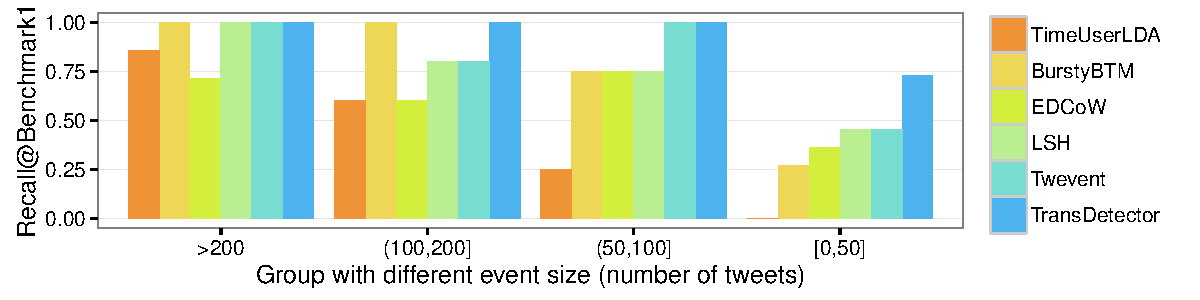
\includegraphics[width=1.0\columnwidth]{img/barchartOnBenchmark1.pdf}
        \caption{The relation between the recall and the event size}
        \label{fig:Benchmark1}
\end{figure}


\begin{table}
\setlength{\abovecaptionskip}{0.cm}%set the distance between caption and table to 0 cm.
\setlength{\belowcaptionskip}{0.cm}
\centering
\caption{Events about \textit{military} detected by systems between 2011-07-22 and 2011-07-28}
\label{my-label}
\scalebox{0.77}{
\begin{threeparttable}  
\begin{tabular}{|c|l|l|c|c|c|c|c|c|c|}
\hline
\multirow{2}{*}{Date} & \multirow{2}{*}{Event key words} & \multirow{2}{*}{Representative event tweet} & \multirow{2}{*}{\begin{tabular}[c]{@{}l@{}}Number of \\ event tweet\end{tabular}} & \multicolumn{6}{c|}{Methods\tnote{a}} \\ \cline{5-10} 
 &  &  &  & L & TU & TW & E & B & TD \\ \hline
7/22/11 & \begin{tabular}[c]{@{}l@{}}Norway, Oslo,\\ attacks, bombing\end{tabular} & \begin{tabular}[c]{@{}l@{}}Terror Attacks Devastate Norway: A bomb ripped through \\ government offices in Oslo and a gunman... http://dlvr.it/cLbk8\end{tabular} & 557 & \checkmark & \checkmark & \checkmark &  &  &  \\ \hline
7/23/11 & Gunman, rink & \begin{tabular}[c]{@{}l@{}}Gunman Kills Self, 5 Others at Texas Roller Rink \\ http://dlvr.it/cLcTH\end{tabular} & 43 & \checkmark & - &  &  &  &  \\ \hline
7/26/11 & \begin{tabular}[c]{@{}l@{}}Kandahar, mayor, \\ suicide, attack\end{tabular} & \begin{tabular}[c]{@{}l@{}}TELEGRAPH{]}: Kandahar mayor killed by Afghan suicide \\ bomber: The mayor of Kandahar, the biggest city in south \_\end{tabular} & 47 & \checkmark & - &  &  &  &  \\ \hline
7/28/11 & Ft., Hood, attack & Possible Ft. Hood Attack Thwarted http://t.co/BSJ33hk & 52 & \checkmark & - &  &  &  &  \\ \hline
7/28/11 & \begin{tabular}[c]{@{}l@{}}Libyan, rebel, \\ gunned\end{tabular} & \begin{tabular}[c]{@{}l@{}}Libyan rebel chief gunned down in Benghazi \\ http://sns.mx/prfvy1\end{tabular} & 44 & \checkmark & - &  &  &  &  \\ \hline
\end{tabular}

\begin{tablenotes}  
\item[a] L=LSH\cite{Petrovic:2010uj}, TU=TimeUserLDA\cite{Diao:2012wj}, TW=Twevent\cite{Twevent2012}, E=EDCoW\cite{Weng:2011wz}, B=BurstyBTM\cite{Yan:2015wm}, TD=\textsc{TransDetector}.
\end{tablenotes}  
\end{threeparttable}  
}
\end{table}


\begin{comment}
Table 1 reports the number of events
detected, the precision and recall, of the three methods respectively.
The results of EDCoW are reproduced from [21]9
. Shown in the
table, our proposed method Twevent yields the best precision of
86.1\% which is significantly larger than the precisions achieved
by EDCoW and Tweventu. Observe that our method Twevent detects
101 events with a recall of 75 realistic events. On the same
dataset, EDCoW detects 21 events in total with 13 realistic events.
Tweventu yields a slighter worse precision than EDCoW (75.3%
vs 76.2\%) but detects the largest number of realistic events. In
terms of DERate, Twevent achieves the lowest rate despite that our
method detects much more events than EDCoW (101 vs 21). On
the other hand, we observe that Tweventu delivers the worst DERate,
more than double of Twevent (41\% vs 16.0\%). That is, the unigrams
about the same event are clustered into two or more events.
Because a tweet segment usually conveys very specific information,
the tweets containing the tweet segment are all about the same
topic (e.g., the event). Two tweet segments about the same event
are therefore have higher chance to be clustered together.
\end{comment}

%An accurate recent states learning leads to accurate event detection.
\begin{comment}
These methods work in four ways. 
1) Based on topic model, BurstyBTM and TimeUserLDA detect bursty topics. 
Although they are designed for batch learning initially, we run them on the slide windows to adapt to the text stream environment.
2) Integrated with knowledge base, Twevent detects bursty segments, groups them into clusters, and then filters out the meaningless ones by Wikipedia.
3) By clustering articles, UMass System and LSH decide whether the article belongs to the existing event or a new one.
As designed for First Story Detection task (one of the Topic Detection and Tracking subtasks\cite{allan2012topic}) initially, they prefer to enlarge the recall of detected events. 
4) By analyzing word frequencies, EDCoW clusters the bursty words into events.
\end{comment}

\begin{comment}
20-newsgroup\footnote{http://qwone.com/~jason/20Newsgroups/}
\end{comment}

\section{Conclusions \& Future Work}
Knowledge base is constructed elaborately and contains rich information, which can benefit the not-well-organized text stream. 
As a part of our future work, we will explore the effects of transfer learning from knowledge base to text stream for more tasks, such as text classification and key words extraction, especially for short texts. 
%Another work what we are interested in is to utilize the knowledge base Microsoft Academic Graph, which also contains the taxonomy structure and text contents, to mine the research topics and trends from arXiv stream in fine grain. 

\begin{comment}
Twitter, as a new type of social media, has experienced an explosive growth in terms of both users and information volume in recent years. 
The characteristics of tweets propose severe challenges to many tasks including event detection. 
In this paper, we present a novel event detection system for Twitter stream, called Twevent, to tackle the adverse impacts of tweets: short and noisy content, diverse and dynamic topics, and large data volume. 
One of the key concept in Twevent is to use tweet segment instead of unigram for identifying the bursty features and then distinguishing the realistic events from the noisy ones. 
Twevent demonstrates outstanding performance in our experiments: effectiveness, informativeness, and efficiency. 
As a part of our future work, we will investigate the effectiveness of utilizing more features from tweets (e.g., retweet rate and hashtags) in Twevent. 
Another important task is to investigate the effectiveness of Twevent when none of the segments of an event is covered by Wikipedia.
\end{comment}

\newpage
\bibliographystyle{unsrt}
\small
\bibliography{paperbib}


\end{document}
